\documentclass[a4paper,10pt]{article}

\usepackage{ifpdf}
\ifpdf
  \usepackage[pdftex]{graphicx}
  \graphicspath{{images/}}
\else
  \RequirePackage[dvipdfm, CJKbookmarks, bookmarks=true, bookmarksnumbered=true%
                unicode,%
             colorlinks,%
         linkcolor=blue,%
             hyperindex,%
       plainpages=false,%
      pdfstartview=FitH]{hyperref}
  \AtBeginDvi{\special{pdf:tounicode UTF8-UCS2}}
  \usepackage[dvipdfm]{graphicx}
  \graphicspath{{images/}}
  \DeclareGraphicsExtensions{.eps}
\fi

%\RequirePackage{CJKutf8,CJKnumb,CJKulem}
\RequirePackage{CJKutf8,CJKnumb}
\RequirePackage{color,verbatim,cite}
\RequirePackage{texnames,makeidx,indentfirst}
\RequirePackage{amsmath,amssymb,amsfonts,bm,manfnt}
\RequirePackage{fancyhdr,titlesec,datetime}
\RequirePackage{wasysym,longtable,multirow,bigstrut}
\usepackage[section]{placeins}
\usepackage[left=3.2cm,right=2.54cm,top=3.3cm,bottom=2.6cm]{geometry}
\usepackage[caption=false,font=footnotesize]{subfig}

\AtBeginDocument{\begin{CJK*}{UTF8}{song}\CJKtilde\CJKindent\CJKcaption{utf8}}
\AtEndDocument{\end{CJK*}}

\setlength{\parskip}{0.75ex plus .2ex minus .5ex}
\renewcommand{\baselinestretch}{1.2}

\hypersetup {
    pdftitle={无线传感器网络中的位置感知安全服务},
    pdfauthor={杨文博}
}

\title{无线传感器网络中的位置感知安全服务}
\author{杨文博}

\begin{document}

\maketitle

\section{ 选题依据 } 

\subsection{课题的研究意义和国内外研究的概况}

\subsubsection{无线传感器网络及其中的安全问题}  

无线传感器网络(Wireless Sensor Network, WSN)在最近几年获得了全球的广泛关注。伴随着与传感器相关的通信、嵌入式和分布式计算技术的飞速发展,特别是微机电系统(Micro-Electro-Mechanical, MEMS)的长足进步,人们研制出了各种不同共用的廉价微型传感器。这些传感器可以感知、测量并收集所处的环境信息,并将这些信息通过某种方式传输给布置无线传感器网络的用户。它们可以被广泛应用于国防军事、国家安全、环境监测、火灾预警、交通管理、医疗卫生和灾难救援等许多领域,帮助人们获得大量有价值的目标环境信息。

无线传感器节点一般情况下由感应模块、处理器、内存、能量供应、无线模块和控制单元组成。装配着不同的感应模块的传感器可以感应物理环境的不同信息,例如湿度、温度、压力、震动、风速、声音、辐射、有毒气体含量等等。由于其廉价性和微型化,无线传感器所采用的处理器一般比较低端,不支持如浮点运算、多媒体指令等一些高级功能。无线传感器节点一般都只有少量的内存,它所收集到的信息将使用无线方式传输到基站。一般情况下,无线传感器节点的能源主要由电池供应,后备能源可以根据环境的不同采用太阳能等其它的能量供应方式。

无线传感器网络则是由大量无线传感器节点构成的分布式、自组织的无线网络。典型的无线传感器网络一般由数十到数千个无线传感器节点组成,用来检测一定范围区域内的环境信息。受无线传感器节点体积小、数量大、资源受限的限制,无线传感器网络往往具有以下特点:

\begin{enumerate}

\item 树形路由、多跳转发。无线传感器网络需要将收集到的信息传回基站,所以一般构成以基站为根节点的树形结构;由于信号的覆盖范围受限,无线传感器节点间通信往往需要经过多跳转发,其转发由传感器节点完成,没有专门的路由设备。

\item 无线传输的带宽、稳定性和安全性较差。由于底层采用无线通信,受到信道本身物理特性的限制,无线传感器网络的通信质量和稳定性往往较差;考虑到无线信号的开放性,其更容易受到信道窃听、伪装、拒绝服务等攻击,需要特别考虑一些安全需求。

\item 网络资源受限。无线传感器网络中,无线节点往往不具有长期的电源供应,节点设计的计算能力、存储空间都要比一般的有线网络节点要小得多。在设计网络网络结构时需要特别考虑到能耗因素,避免部分节点能源耗尽导致整个网络失灵。

\end{enumerate}

\begin{figure}[htbp]
  \centering
  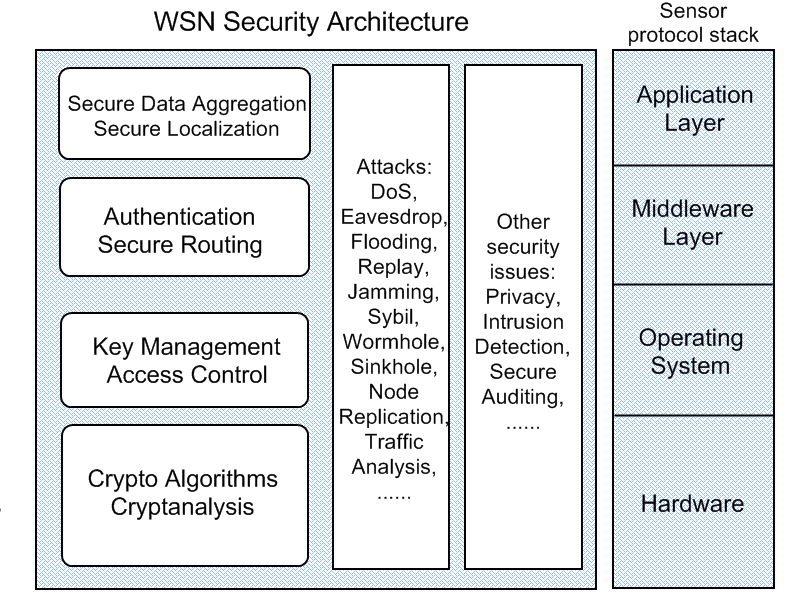
\includegraphics[width=0.8\textwidth,keepaspectratio]{wsn_sec_map}
  \caption{\label{wsn_sec_map}无线传感器网络安全架构~\cite{Li2005}}
\end{figure}

由于受以上条件限制,很多传统的安全措施难以使用在无线传感器网络上,而且无线传感器网络往往用于监测敏感信息或者部署在充满敌意的环境中,所以无线传感器网络在应用中面临很多安全问题~\cite{Xiao2006}:

\begin{enumerate}

\item 数据安全。在无线传感器网络中,数据的安全需求包括数据的保密性、完整性和新鲜性。数据的保密性需求包括节点数据不泄露给其它节点、密钥分配的信道安全以及抵抗流量分析;数据的完整性要求在传输的过程中数据不被恶意节点篡改;数据的新鲜性要求数据通信能抵抗重放攻击,识别收到的包是否是最新的数据。

\item 网络可用性。由于计算量以及能量消耗过大,重量级的密码学方法无法使用在无线传感器网络中。如何剪裁密码学方法,有效重用资源,或者引入轻量级的保密方案,在资源消耗和安全保证之间保持一定的平衡是迫切需要解决的问题。

\item 安全组网。无线传感器网络属于自组织网络的范畴,所以节点在组网的时候必须保证能够支持多跳路由,还需要考虑到自组织的密钥管理的方法。

\item 时钟同步。为了节省能量,无线传感器节点需要在不通信的时候保持休眠状态,这就要求在无线传感器之间有某种同步机制,比如通信双方同步,多跳同步和组同步。

\item 安全定位。当无线传感器节点的某部分出故障时,往往需要对故障的节点或者部分做自动的精确定位,但是当恶意节点存在时,攻击者可以操作定位信息来误导其它节点。对故障部分的安全定位需要引入专门的算法来消除恶意节点的影响。

\item 安全认证。由于无线传感器网络的开放性,恶意节点可以伪装自己加入传感器网络,并发送错误的数据,所以必须在无线传感器网络中加入认证机制来保证消息来自网络中真实正确的数据源。

\end{enumerate}

\section{研究内容和研究方法} 

研究内容、拟采用的研究方法、技术路线等方面有哪些创新之处。

\section{课题研究的创新之处}

a

\section{研究工作进度安排}

a

\section{已取得的与论文研究内容相关的成果} 

无。

\bibliographystyle{IEEEtran}
\bibliography{wsn}

\end{document}

